\documentclass[nopalatino,nolot,nolof,color,11pt]{fithesis3}
\thesissetup{
  faculty=fi,
  type=mgr,
  author={Bc. Pavel Dedík},
  advisor={doc. Mgr. Radek Pelánek, Ph.D.},
  title={Modeling Human Memory for Adaptive Educational Systems},
  keywords={Memory, Learning, Forgetting, Knowledge, Machine Learning, Student Modeling, Performance Factor Analysis}}

\usepackage{lmodern}
\usepackage{amssymb}
\usepackage{graphicx}
\usepackage{enumitem}
\usepackage{algorithm}
\usepackage{mathtools}
\usepackage{subcaption}
\usepackage{booktabs,siunitx}
\usepackage[noend]{algpseudocode}

% To be removed when the thesis is finished.
\usepackage{lipsum}

\setlist[itemize]{leftmargin=10mm}

\begin{document}
  \chapter{Introduction}

Memory could be defined as the biological storage for the information acquired from past experience with the environment. Human memory has been scientifically studied for at least 100 years~\cite{baddeley1997human} and today we know that there are many types of memory, all cooperating in the process of memorization so that they could be used to govern subsequent behavior of each individual. Memory is not a single unitary system such as the heart, but a collections of systems where one system is responsible for the encoding of new information while another system helps with its storage over a long period of time. The systems responsible for retention of information in the human brain are also very closely related to \textit{learning} and \textit{forgetting}, both of which in turn depend to some extent on memory. That is true because our memory provides the means and structure to link new knowledge faster by association and inference. Hence, human memory is a \textit{complex system} and the whole underlying process is still broadly studied by researchers who try to understand the complex cognitive processes by exploring the different memory systems of animals (e.g. rats) or patients who suffer amnesia as a consequence of brain damage~\cite{mcclelland1995there}.

The exploration of human memory and learning has applications particularly in education, where our goal is to increase the amount of material students learn in one study session. Before the invention of computers and the growth of the Internet, the ways to test and evaluate new methods of educating students involved classrooms with usually only a limited number of participants. In the last 20 years, students and educational institutions started to use and develop new e-learning systems as a complimentary tool for education. \textit{Adaptive educational systems} (sometimes referred as adaptive practice systems) are systems that provide online environment for practicing different domains of educational content adaptively.

In adaptive educational systems, our effort is to create sufficiently accurate representation of students in order to make the system personalized, increase students' motivation and the speed of learning. A part of all adaptive systems are mathematical models which are constructed in order to model learning of individual students and adapt the system to students' abilities, behavior and knowledge of the subject. These models and their evaluation is very often based on \textit{machine learning} techniques and is closely related to statistics. The ability to model the adaptive behavior also requires research connected to cognitive psychology.

One example of a free web-based adaptive educational system is the project called Outline Maps\footnote{Available at \href{http://outlinemaps.org}{\texttt{outlinemaps.org}}} developed at the Faculty of Informatics at Masaryk University. This project helps students practice all kinds of geography facts~\cite{Papousek2014}, including world countries, cities, rivers, lakes, mountains, islands, Czech regions, and many others. The practice procedure of geography in the system involves rehearsal of contextual information about a place on a map, i.e. the location, shape or neighbors of a country. The test of students' knowledge is done by presenting questions requiring the identification of correct association between a name of a place and its position on an outline map (see Figure~\ref{fig:slepemapy}).

\begin{figure}[htbp]
  \centering
  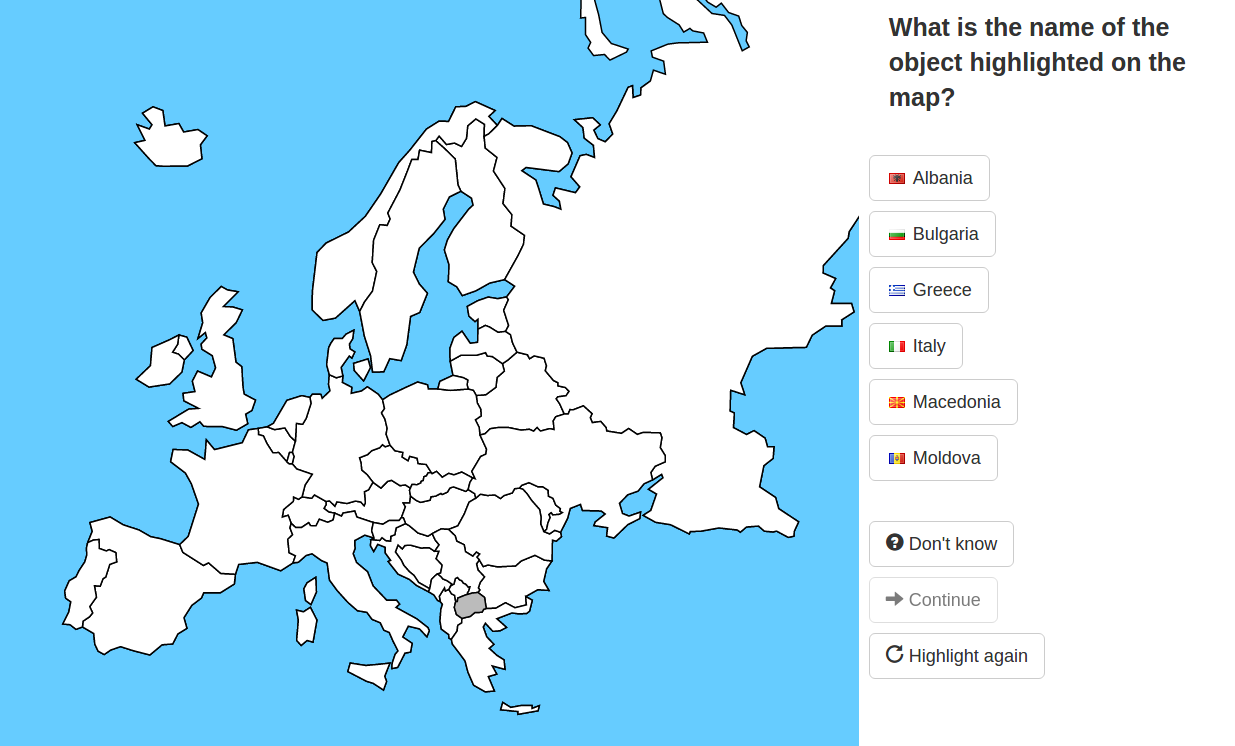
\includegraphics[width=\textwidth]{img/slepemapy}
  \caption{The screenshot corresponds to a multiple-choice question (with 5 distractors) requiring the student to identify the name of the highlighted country on an outline map of Europe.}
  \label{fig:slepemapy}
\end{figure}

Since the system is adaptive, it examines knowledge and skills of students adaptively based on previous answers---by the selection of optimal repeat frequency, the type of question, its difficulty etc. In this context, the practice of geography is somewhat different from ordinary memorization of vocabulary pairs as there are bigger variations in the prior knowledge of individual students.

\section{Objectives}

The first objective of the thesis is to study the related research to modeling human memory and forgetting mainly in the context of adaptive educational systems. The first objective also involves the study of the relevant machine learning models and the determination of which one is the best candidate considering all its aspects.

Our primary objective is to design, evaluate and analyze the models suitable for adaptive practice systems while accounting for key aspects of human memory and forgetting. The findings should provide insights into how modeling the effect of forgetting improves model's performance. We are particularly interested with student modeling for application in the adaptive system Outline Maps.

\section{Outline}

The second chapter covers the background of our thesis, we summarize the most relevant attributes of human memory and forgetting that are related to our research, we also describe characteristics of adaptive educational systems as well as mathematical models used in student modeling. In the third chapter, we propose models and their modifications that focus on \textit{timing information} (e.g. the ages of student's past trials and response times), we also describe the methods commonly used in machine learning for parameter estimation and metrics for the quantification of model's performance. The fourth chapter includes evaluation of the proposed models and further analysis of their parameters. Finally, the last chapter concludes the results of our experiments and outlines suggestions for possible future research.

  \chapter{Background}

In this chapter we present an overview of the related research with the topic of our thesis. Firstly, we describe how the human brain can acquire new knowledge, the process of retention of information and the retrieval of information from memory. Secondly, we give an overview of the techniques suitable for educational systems with the focus on adaptive learning of facts.

\section{Student Modeling and Memory}

Throughout the last one hundred years, researchers have been trying to figure out the complex cognitive processes in the human brain responsible for our ability to learn~\cite{RichardE.Mayer2010}. Understanding the process of learning can be very helpful in education and educational systems where we wish to improve the student's representation in order to be able to better adapt to the needs and knowledge of an individual student practicing a particular domain (e.g. the knowledge of animals, Japanese vocabulary or geography). The construction of a quantitative representation, called a \textit{student model}, is known as \textit{student modeling}~\cite{Sison1998}.

The Greek philosopher and mathematician Plato compared human mind to an aviary in which each bird represented a memory~\cite{MichaelW.Eysenck2008}. Today, we have a much better intuition on the human biological storage -- the hardware responsible for the storage and organization of data in modern computers. This analogy of computer data storage is much better than the one Plato used and it seems to be very close and accurate depiction of the human memory.

So far, we haven't mentioned learning, which is very closely related to memory and to the topic of our thesis. Learning leads to the creation of memory. The study of learning and memory can be divided even further when we realize that we need some way to observe what the students know by experiments. This section is thus explained in three parts:

\begin{itemize}
  \item Learning
  \item Memory
  \item Performance
\end{itemize}

In a book released by a professor of psychology at the University of California Richard~E.~Mayer, the science of learning is organized into three components, that is the science of:

\begin{itemize}
  \item Learning
  \item Instruction
  \item Assessment
\end{itemize}

All of these components are to some extent related to our research. However, the science of learning is the most related since it concerns human memory and learning. The science of instruction is about the manipulation of the student's environment in order to foster learning, it's the scientific study of how to help people learn. In educational systems, this is usually done by incorporating \textit{instructional policies}, the strategies or a set of instructions that help students maintain engagement and increase the amount gained knowledge in one session, instructional policies guide students during learning (e.g. by the selection of appropriate questions or the number of options in multiple-choice tests). Lastly, the science of assessment seeks to determine what people know, which is important so that we are able to quantify the effectiveness of different instructional methods~\cite{RichardE.Mayer2010}.

\subsection{Learning}

\begin{figure}[htbp]
\centering
  \begin{subfigure}{.49\textwidth}
    \centering
    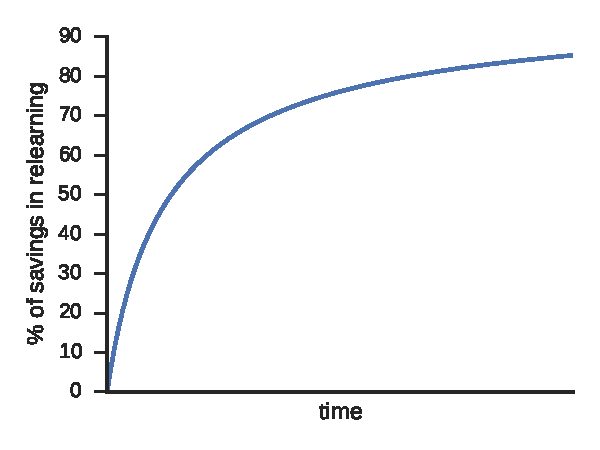
\includegraphics[width=\textwidth]{img/learning-curve}
    \caption{Learning curve}
    \label{fig:learning-curve}
  \end{subfigure}
  \begin{subfigure}{.49\textwidth}
    \centering
    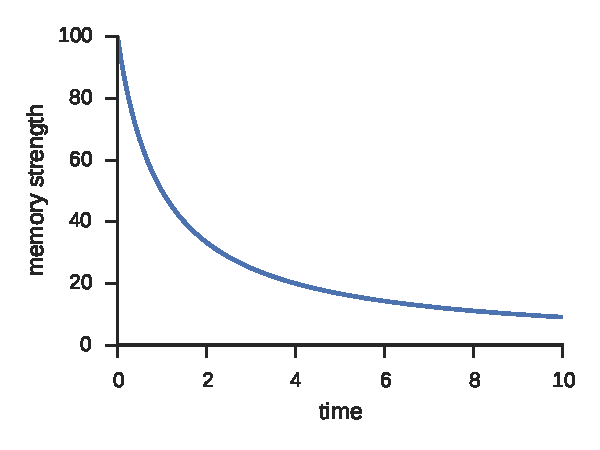
\includegraphics[width=\textwidth]{img/forgetting-curve}
    \caption{Forgetting curve}
    \label{fig:forgetting-curve}
  \end{subfigure}
% \caption{Learning curve (left) and forgetting curve (right).}
\label{fig:learning-forgetting-curves}
\end{figure}

Richard E. Mayer formulated learning as a change in what the learner knows caused by the learner's experience~\cite{RichardE.Mayer2010}. More specifically, learning is the process of encoding, modifying and reinforcing information~\cite{Lewis}. For example the encoding of the location of Portugal can be seen as learning the shape of the country, its neighbor Spain and the surrounding ocean.

A learning curve is the rate of the student's progress in gaining new skill or knowledge by experience in the environment (e.g. by participating in a discussion, reading a book or riding a bike). Generally, the change in learner's skill or knowledge is proportional to the product of amount learned and amount to yet learn. Several functions modeling the learning curve were proposed in the past, namely the power law, exponential and hyperbolic function. Even though some researchers believe in a bias introduced by averaging many trials during the evaluation of the function, learning is widely believed to follow the power law~\cite{Klusasek2014}.

In order to be able to model learning we need to be able to measure \textit{memory strength}, which is just a measurement of the ability to retrieve an item from memory. Memory strength can be measured indirectly by observing the following attributes of students when an item is practiced:

\begin{description}[leftmargin=0cm]
  \item[Probability of recall] Probability of the student recalling the practiced item, which can be measured as the fraction of the number of successful recollections and the number of all presentation of the specific item.
  \item[Latency of recall] Latency of the student when retrieving the practiced item from their memory. Latency of recall can be measured by observing the response times of students.
  \item[Savings in relearning] The number of required revisions of the practiced item in order to fully regain its knowledge~\cite{MichaelW.Eysenck2008}.
\end{description}

We can further distinguish the following levels of learning as measured by memory strength:

\begin{description}[leftmargin=0cm]
  \item[Familiarity] The student has feeling they knew the item in the past but cannot remember anymore.
  \item[Recognition] The student recognized the item when presented multiple-choice options but couldn't remember otherwise.
  \item[Recall] The student is able to recall the item with some effort. Note that cognitive science distinguishes \textit{free recall} and \textit{cued recall}. Free recall is the ability to remember the item without any help (e.g. recalling the name of a country), in the case of cued recall, we are given an information which can help us remember (e.g. first letter of the country we are to remember).
  \item[Automaticity] The student recalls the item instantaneously when presented. Note that the level of automaticity can be measured by the latency of recall.
\end{description}

\subsection{Memory}

Memory is the biological storage that retains the information, e.g. the location of Portugal. The student's memory, however, decays with time. This memory decay is called \textit{forgetting} and similarly as learning it respects the power law.

Forgetting can be reduced by repetition. Repetition can be massed or spaced. In a massed presentation the item is revised in a short interval many times over. In contrast, a spaced presentation usually consists of revisions performed in a longer period of time with pauses between presentations. It is well known that a spaced presentation leads to a better memory strength~\cite{RichardE.Mayer2010}. This phenomenon is called the \textit{spacing effect}.

The long-term memory of humans can be thought as:

\begin{itemize}
  \item Procedural (knowing how)
  \item Declarative (knowing what)
\end{itemize}

The procedural memory goes beyond our conscious awareness and makes us capable of the incremental acquisition of both the motor and cognitive skills. The declarative memory (sometimes referred as explicit memory) is the conscious knowledge such as the world's countries or the English vocabulary~\cite{MichaelW.Eysenck2008}.

\subsection{Performance}

The performance of students is the determination of what they know. Performance can be estimated from the speed and precision of recall, e.g. by a multiple-choice test, where the correctness of answers and response time is measured~\cite{Lewis}. Performance can be seen as an instrument that describes the student's knowledge, the understanding of which is important because it helps us guide the instructional policy.

\section{Relevant Student Models}
\label{relevant-models}

In this section we discuss the models relevant to our work. There are two main components that concern us. The first is the estimation of prior knowledge which can be helpful if we need better understanding of the student's acquired knowledge. The second is the estimation of the current knowledge which combines the knowledge the student already had and the knowledge they acquired. Estimation of current knowledge is significant for the better part of this thesis.

\subsection{Elo System}
\label{elo}

Elo system is a mathematical model suited for student modeling as recent research has shown. Elo rating system and its extension Glicko is otherwise a very popular approach in competitor-versus-competitor games such as chess~\cite{Vanek2014}. In our work we employ the model for the estimation of prior knowledge of students.

In the standard version of Elo system we have the student's skill $\theta_s$ and the difficulty of an item $b_i$. Equations~\ref{eq-elo-skill} and~\ref{eq-elo-difficulty} demonstrate an update of the student's skill and the item's difficulty after one answered question. The parameter $R$ is $0$ or $1$ depending on the correctness of the student's answer. The probability that a student with a given skill $\theta_s$ will answer correctly on the presented question of difficulty $b_i$ is estimated by a logistic function (see Equation~\ref{eq-elo-logistic}).

\begin{equation} \label{eq-elo-skill}
  \theta_s \gets \theta_s + K(R - P(R = 1|s,i))
\end{equation}

\begin{equation} \label{eq-elo-difficulty}
  b_i \gets b_i - K(R - P(R = 1|s,i))
\end{equation}

\begin{equation} \label{eq-elo-logistic}
  P(R = 1|s,i) = \frac{1}{1 + e^{-(\theta_s - b_i)}}
\end{equation}

The constant parameter $K$ affects the change in the estimates $\theta_s$ and $b_i$. Higher value means faster change after few questions, in contrast lower value makes the change slower. This is a problem since the number of answers varies throughout the time. It's been demonstrated that the use of an uncertainty function $\frac{a}{1 + bn}$, which considers the number of answers of students in the system, makes the predictions more stable and increases accuracy~\cite{Vanek2014}.

\subsection{Performance Factor Analysis}
\label{pfa}

Performance Factor Analysis (PFA) is a student modeling approach based on the Learning Factor Analysis (LFA). The standard PFA equation is formulated with the incorporation of knowledge components (KCs), which may include skills, concepts or facts~\cite{Pavlik2009}.

\begin{equation} \label{eq-pfa-standard}
  m(i,j \in KCs,s,f) = \sum_{j \in KCs} \beta_j + \gamma_j s_{i,j} + \delta_j f_{i,j} 
\end{equation}

\begin{equation} \label{eq-pfa-standard-p}
  P(m) = \frac{1}{1 + e^{-m}}
\end{equation}

In Equation~\ref{eq-pfa-standard}, where $m$ is a function of the student's knowledge, the parameter $\beta_j$ is the difficulty of the knowledge component $j$. The counts of current successes and failures of the student $i$ and the knowledge component $j$ are represented by the parameters $s_{i,j}$ and $f_{i,j}$, where $\gamma_j$ and $\delta_j$ define the weight of each success and failure.

The standard PFA model is defined in terms of knowledge components which is not always needed. The main disadvantage, however, is the inability to consider the order of answers. Another problem with the standard model is that it doesn't take into account the probability of guessing. Both these issues are solved in the following model:

\begin{equation} \label{eq-pfa-extended}
  m \gets \begin{cases}
            m + \gamma \cdot (1 - P(m)) & \text{\textbf{if }} \text{the answer was correct} \\
            m + \delta \cdot P(m) & \text{\textbf{otherwise}}
          \end{cases}
\end{equation}

\begin{equation} \label{eq-pfa-standard-p}
  P(m) = \frac{1}{n} + \left(1 - \frac{1}{n}\right)\frac{1}{1 + e^{-m}}
\end{equation}

The initial value of $m$ in Equation~\ref{eq-pfa-extended} can be estimated from the Elo model which was discussed in the section~\ref{elo}, i.e. $m = \theta_s - b_i$. The parameter $n$ in the Equation~\ref{eq-pfa-standard-p} matches the number of options in multiple-choice question. Note that the probability of guess is $\frac{1}{n}$ and the probability of slip is $1 - \frac{1}{n}$.

Another variation of the original PFA model was proposed by Yue Gong~\cite{Gong2011}. The idea of the model is based on the fact that we expect the student who answered in total of four presentations two times correctly in the last two presentations to perform better than the student who answered correctly in the first two presentations. The extended model introduces a decay factor $\xi$ that changes the behavior of the parameters $s_{i,j}$ and $f_{i,j}$ (see Equations~\ref{eq-pfa-gong-s},~\ref{eq-pfa-gong-f}).

\begin{equation} \label{eq-pfa-gong-s}
  s_{i,j} = \sum_{k=1}^{n-1} y_k \cdot \xi^{n-1-k}
\end{equation}

\begin{equation} \label{eq-pfa-gong-f}
  f_{i,j} = \sum_{k=1}^{n-1} |y_k - 1| \cdot \xi^{n-1-k}
\end{equation}

The parameter $y_k$ represents the correctness of the $k$-th question. 
The problem of this model is that it cannot be easily adjusted so that it includes the probability of guessing, particularly in cases where the practices were presented in the form of multiple-choice questions with varied number of options.

\todo{Some examples would be nice.}

\subsection{Models of Students' Memory}
\label{spacing-effect}

\todo{Nice plot showing what the hell this is all about.}

In the ACT-R model~\cite{Pavlik2003}, the memory strength $m$ of the student $s$ can be modeled by the Equation~\ref{eq-actr}.

\begin{equation} \label{eq-actr}
  m_n(t) = \ln{\sum_{i=1}^{n} t_{i}^{-d}}
\end{equation}

The parameter $t$ is a vector of seconds that passed since each of the $n$ repetitions were performed by the student $s$. The parameter $d$ represents memory decay (the speed of forgetting). Note that the equation is just a simplification of the reality and does not take into account many very important aspects of forgetting, e.g. the mentioned spacing effect.

Philip~I.~Pavlik and John~R.~Anderson~\cite{Pavlik2005} developed an extended version of the equation in which the decay is a function of the activation at the time the item was presented (see Equation~\ref{eq-pavlik-decay} and Equation~\ref{eq-pavlik-activation}).

\begin{equation} \label{eq-pavlik-decay}
  d_i = ce^{m_{i-1}} + a
\end{equation}
\begin{equation} \label{eq-pavlik-activation}
  m_n(t) = \ln{\sum_{i=1}^{n} t_{i}^{-d_i}}
\end{equation}

The parameters $c$ and $a$ affect the scale of the decay. Since $m_0 = -\infty$, the value of $d_i$ is always equal to $a$ for the first practice of the student. Additionally, when $c = 0$, the result of the equation is equivalent with the Equation~\ref{eq-actr}. Because the computation is recursive and a bit complex, we present the pseudo-code of the algorithm computing the memory activation function (see Algorithm~\ref{alg-memory-activation}).

\begin{algorithm}
  \caption{The function $\textsc{MemoryActivation}: \mathbb{N}^n \rightarrow \mathbb{R}^n$ takes the vector parameter $t$ in descending order, e.g. $[56800, 56400, 3600, 60, 0]$ (the last zero is the current practice). The result of the computation is a vector $m$ of student's memory strengths during each practice.}
  \label{alg-memory-activation}
  \begin{algorithmic}[1]
    \Function{MemoryActivation}{$t$}
      \State $n \gets size(t)$
      \State $m_0 \gets -\infty$
      \For{$i \gets 1$ \textbf{to} $n-1$}
        \State $s \gets 0$
        \For{$j \gets 1$ \textbf{to} $i$}
          \State $d_j \gets ce^{m_{j-1}} + a$
          \State $s \gets s + (t_j - t_i)^{-d_j}$
        \EndFor
        \State $m_i \gets \log(s)$
      \EndFor
      \State \Return $m$
    \EndFunction
  \end{algorithmic}
\end{algorithm}

\todo{Proof of correctness? Perhaps not necessary.}

Note that the time complexity of the function is $\mathcal{O}\left(\frac{n(n-1)}{2}\right)$.

  \chapter{Models and Methods}

The models presented in chapter~\ref{relevant-models} seem to work well either in the context of adaptive systems where we aren't concerned with timing information or have been tested in controlled environment where the students had no prior knowledge of the presented material. In this chapter, we elaborate the methods we used to further improve the performance by taking into account the timing information of students' answers, i.e. the response times or the breaks between presentations (the timing distance). We are interested primarily in domains where the prior knowledge varies widely between students.

\section{Models Based on Timing Information}

In this section we discuss several models which aim at modeling students' memory with the usage of timing information of answers. There are several issues to consider beforehand:

\begin{itemize}
  \item Students have different skills and thus the rate of retention loss varies.
  \item The difficulty of items varies, some items are forgotten faster and some slower.
  \item The prior knowledge of each student is different. If the student already learned the practiced item and has it stored in their long term memory, the process of forgetting is much slower.
\end{itemize}

\subsection{The Extended Model}
\label{pfaet}

The PFA Extended model summarized in chapter~\ref{pfae} can be further enhanced when we utilize the timing information by locally changing the memory activation in prediction. The difference in seconds between the times of the current question and the last answer is passed to a \textit{time effect function} (we adapted this term from a related work~\cite{Pelanek2015}). The time effect function increases or decreases the probability of recall or the memory activation depending on the timing distance. The updated equation with a time effect function is depicted in Equation~\ref{eq-pfa-standard-time-p}.

\begin{equation} \label{eq-pfa-standard-time-p}
  P(m) = \frac{1}{1 + e^{-(m + f(t))}}
\end{equation}

The advantage of this model is that it shares the same properties as the presented PFA Extended model, i.e. it's straightforward to employ Elo model for estimation of prior knowledge as well as to account for the probability of guessing.

\subsection{The Alternative Model}
\label{pfagt}

Another way of dealing with timing distances between attempts is by changing the decay factor $\xi$ of the model presented in chapter~\ref{pfag}. The model takes into account the order of questions, yet doesn't consider brakes between student's practices of an item. This problem can be resolved by replacing the parameter $\xi$ with a time effect function.

\begin{equation} \label{eq-pfa-gong-time-s}
  s_{i,j} = \sum_{k=1}^{n-1} y_k \cdot f(t_k)
\end{equation}

\begin{equation} \label{eq-pfa-gong-time-f}
  f_{i,j} = \sum_{k=1}^{n-1} |y_k - 1| \cdot g(t_k)
\end{equation}

Equations~\ref{eq-pfa-gong-time-s} and~\ref{eq-pfa-gong-time-f} show the incorporation of the time effect function $f$ and $g$ in the model. The parameter $t_k$ represents the number of seconds that passed between the $k$-th practice and the most recent one. The weight of successes and failures is thus dependent on the ages of the prior practices.

As was discussed in the chapter~\ref{pfa}, the problem arises with multiple-choice questions. Another complication is the choice of some good time effect functions that fit the data well. Note that in this model, we often set $\gamma = \delta = 1$, the weight of each success and failure is then entirely dependent on the parameters of the chosen time effect functions instead of $\gamma$ and $\delta$.

\subsection{The Response Time}
\label{pfart}

The response time of student may indicate student's level of learning. If the student answers quickly, it often implies the level of automaticity. We address this phenomenon by increasing the memory activation $m$ after each answered item.

\begin{equation} \label{eq-pfa-extended-rt}
  m \gets \begin{cases}
            m + \gamma \cdot (1 - P(m)) + r(t_d), & \text{\textbf{if }} \text{the answer was correct} \\
            m + \delta \cdot P(m) + r(t_d), & \text{\textbf{otherwise}}
          \end{cases}
\end{equation}

Equation~\ref{eq-pfa-extended-rt} shows the adjusted update rule with a unary function $r(t_d)$, the parameter $t_d$ is the difference between the time the item was presented and the time it was answered (i.e. it's the student's delay).

\section{Quantifying the Quality of Predictions}

One way to quantify the quality of model predictions is to use metric functions. A good choice of a metric function is important for accurate evaluation of performance of student models. In our case we aren't interested strictly in the correctness of student's answers, the goal is to precisely assess their knowledge. The information of student's knowledge is crucial if we don't want to demotivate the student by too difficult or simple questions. For this purpose a good choice is the Root Mean Squared Error metric (see~Equation~\ref{rmse}) or the less popular Log Likelihood (see~Equation~\ref{ll})~\cite{Pelanek2015a}.

\begin{equation} \label{rmse}
  RMSE = \sqrt{\frac{\sum_{i=1}^n (p_i - y_i)^2}{n}}
\end{equation}

\begin{equation} \label{ll}
  LL = \sum_{i=1}^n y_i \log(p_i) + (1 - y_i) \log(1 - p_i)
\end{equation}

The RMSE metric represents ``error'', its the square root of the sum of all squared differences between predicted values $p_i$ and true values $y_i$ divided by the number of samples in data set. RMSE yields a number between 0 and 1, where 0 represents perfect predictions. LL metric is the logarithm of likelihood, the LL value is a negative number dependent on the size of the data set (the bigger the dataset, the lower LL value is possible). Higher values of LL represent the better predictions.

In domains such as information retrieval or pattern recognition other types of metrics are commonly used which are based on qualitative understanding of errors~\cite{Pelanek2015a} instead of their probabilistic value. An advantage of this type of metrics is that it can be easily used in multi-classification tasks. These metrics, however, depend on a chosen threshold, e.g. in case the threshold is set to $0.5$ the predictions $0.51$ and $0.98$ are classified as positive while predictions $0.49$ and $0.04$ are classified as negative.

\begin{table}[htbp]
  \centering
  \caption{Confusion matrix.}
  \begin{tabular}{ l l c c }
   \toprule[\heavyrulewidth]
   & & \multicolumn{2}{c}{\textbf{Predicted Outcome}} \\
   & & Positive & Negative \\
   \midrule[\heavyrulewidth]
   \multirow{2}{5em}{\textbf{Observed Value}}
   & Positive & True Positive (TP) & False Negative (FN) \\
   & Negative & False Positive (FP) & True Negative (TN) \\
   \bottomrule[\heavyrulewidth]
  \end{tabular}
  \label{table:confusion-matrix}
\end{table}

The Table~\ref{table:confusion-matrix} shows the confusion matrix of binary classifier (i.e. the mislabeling of classes). Once the confusion of classes is calculated, we can derivate for example precision (see~Equation~\ref{precision}) and accuracy (see~Equation~\ref{accuracy}).

\begin{equation} \label{precision}
  \mathit{Precision} = \frac{TP}{TP + FP}
\end{equation}

\begin{equation} \label{accuracy}
  \mathit{Accuracy} = \frac{TP + TN}{TP + FP + TN + FN}
\end{equation}

Even though the precision and accuracy aren't very fit in our case as we are more interested in probabilistic understanding of errors, another commonly used metric based on marking predictions as true/false positives/negatives is Area Under the ROC Curve (AUC). In this metric, we measure the performance across all possible thresholds. The result is a number between $0.5$ and $1$, where $1$ represents perfect predictions of the classifier. Note that if all predictions are divided by 2, AUC stays the same, this property is sometimes criticized---hence, it should be used with caution~\cite{Pelanek2015a}.

\section{Parameter Estimation}

The goal of the fitting procedure is to find the optimal parameters that perform well on new samples (in our case predict the student's ability to answer a question correctly). In this section we describe some metrics commonly used for the evaluation of predictive performance (i.e. the fitness of parameters in the model) and the principal algorithms that are suitable for parameter estimation in our case.

\subsection{Grid Search}

This technique is used for parameter optimization, it exhaustively generates a grid of all combinations of selected parameter values where each point in the grid is a function value of a chosen metric (e.g. RMSE). The fittest combination of parameters is represented by the best score of the metric (e.g. has lowest error). The figure~\ref{fig-grid-search-rmse-auc} portrays an example of the grid search on PFA model with two parameters $\gamma$ and $\delta$.

\begin{figure}[htbp]
  \centering
  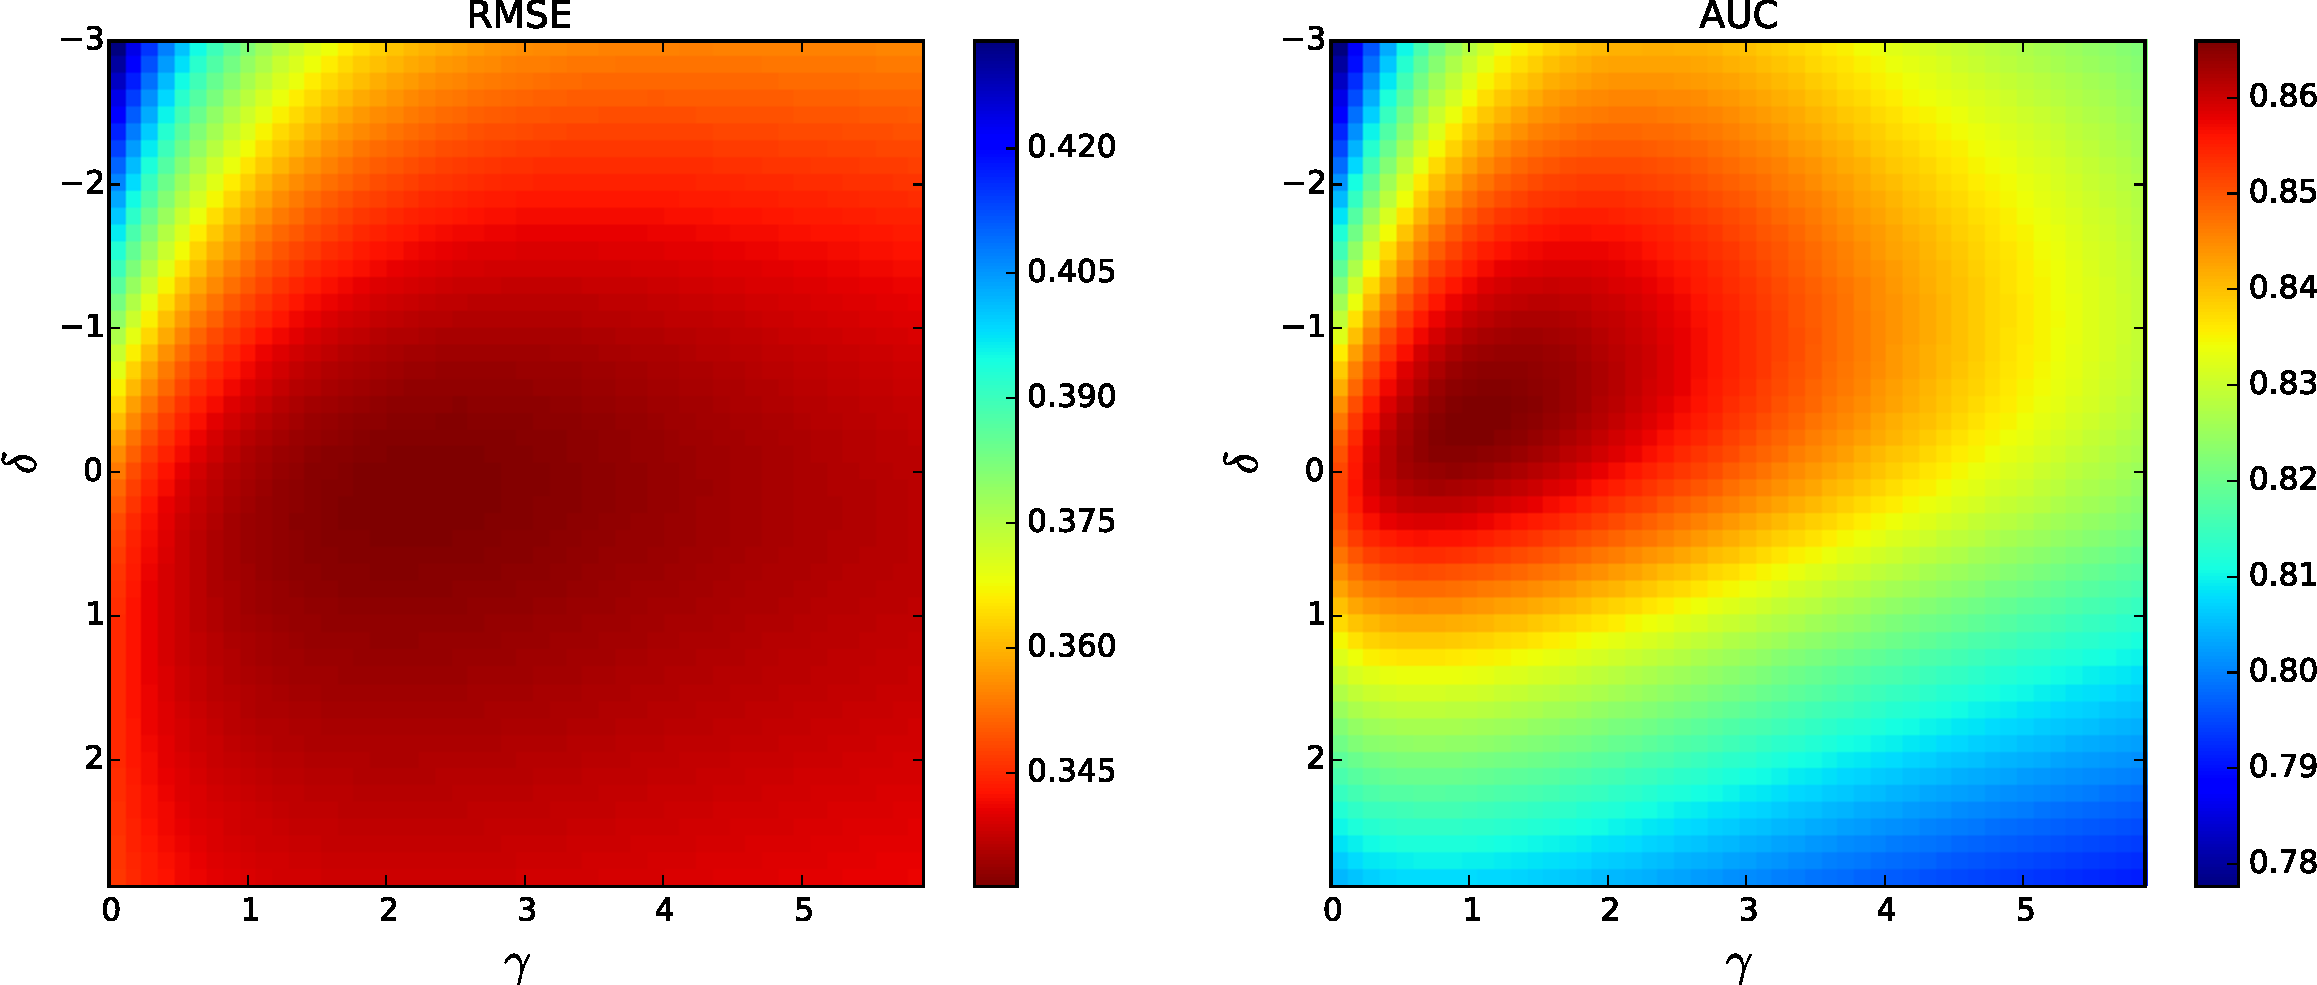
\includegraphics[width=\textwidth]{img/pfa-grid-search-rmse-auc}
  \caption{Result of the grid search performed on the PFAE model.}
  \label{fig-grid-search-rmse-auc}
\end{figure}

The disadvantage of this optimization method is the high computational complexity especially in cases when the model contains a lot of parameters. Also, there is no simple way to plot or visualize a high-dimensional grid.

\subsection{Hill Climbing}
\label{hill-climbing}

This method starts from a given position in the parameter space and evaluates the score of an objective function (metric function in our case). The model is then trained using the values from the enclosing neighborhood of the parameter space, afterwards the best combination of parameters is selected and the process repeated. This continues until there is no other parameter value in the neighborhood with a better score of the objective function, i.e. we found the local minimum~\cite{Russell2009}. TODO: elaborate, maybe write pseudocode, or at least more formal description.

\subsection{Gradient Descent}
\label{gradient-descent}

Gradient descent is optimization algorithm very similar to hill climbing, the difference is that gradient descent has indication which way to ``climb''. The goal of gradient descent is to find the best parameters for a function called hypothesis~\cite{Klusasek2014}, this is done by finding the lowest value of the cost function $J(\rho)$ (similar to objective function in hill climbing). The cost function represents the error of a chosen hypothesis $h_{\rho}(x_i) = \rho^T x_i = \sum^n_{j=0} \rho_j x_{i,j}$, where $\rho_j$ is the value of the $j$-th parameter and $x_{i,j}$ the $i$-th value of the $j$-th feature (e.g. the skill of the student $i$).

\begin{equation} \label{cost-function}
  J(\rho) = \frac{1}{2m} \sum^m_{i=1} (h_{\rho}(x_i) - y_i)^2
\end{equation}

Formal definition of the cost function is depicted in Equation~\ref{cost-function}, it is the sum of all squared errors of hypotheses $h_{\rho}$ over all examples from data set of size $m$ divided by $2m$. Our is to minimize the value of $J(\rho)$ which can be done efficiently by the estimation of the gradient using the following update rule:

\begin{equation} \label{cost-function-update}
  \rho_j \gets \rho_j - \alpha \frac{\partial}{\partial \rho_j} J(\rho)~~\text{for all } j
\end{equation}

The partial derivatives help indicate the surface of the cost function, it gives us the information which direction to take in order to reach the closest local minimum. The value of $\alpha$ is the size of one step or a learning rate, if the value is too big the algorithm might not be able to ever reach a local minimum, in contrast if the value is very small, it is less efficient and the computation takes longer. Now we can imagine that the main difference between gradient descent and hill climbing is that the latter doesn't have any indication of which turn to take next and how big one step in a direction should be~\cite{Russell2009}.

\begin{figure}[htbp]
  \centering
  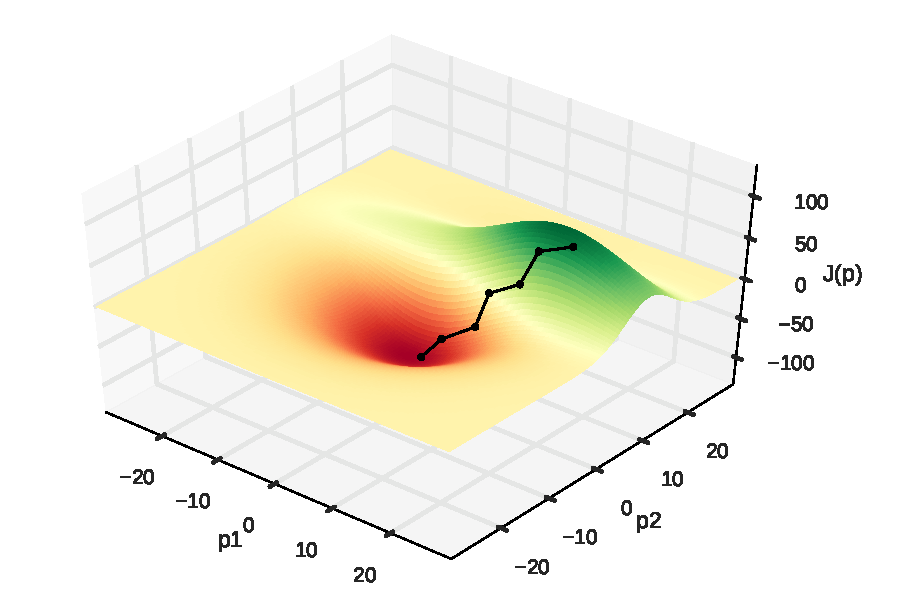
\includegraphics[width=\textwidth]{img/gradient-descent}
  \caption{3D visualization showing first 7 iterations of gradient descent applied to an example with two parameters.}
  \label{fig-gradient-descent}
\end{figure}

\subsection*{Gradient Descent in Online Learning}

In online learning, straightforward way to use optimization methods such as gradient descent doesn't exist. We can, however reuse some aspects of several algorithms used in machine learning and data mining for parameter optimization.

The most obvious and easiest way to implement gradient descent in cases where there is no derivative of the object function could average the difference between observations (correctness of student's answer $y_i$) and predictions (model's predicted probability that the user $i$ answers correctly $p_i$). The batch update rule could be defined as follows:

\begin{equation} \label{online-learning-batch-rule}
 \rho_j \gets \rho_j - \alpha~\frac{1}{n}\sum_{i=0}^n (p_i - y_i)~~\text{for all } j
\end{equation}

It is easy to demonstrate that this method doesn't work well even when the number of parameters is very low. The parameters get easily stuck in the local minimum as can be observed in the Figure~\ref{fig-grid-search-rmse-off}. Another disadvantage of this technique is that we need to relearn the optimal parameters by repeating the process of evaluation periodically on the whole data set.

\begin{figure}[htbp]
  \centering
  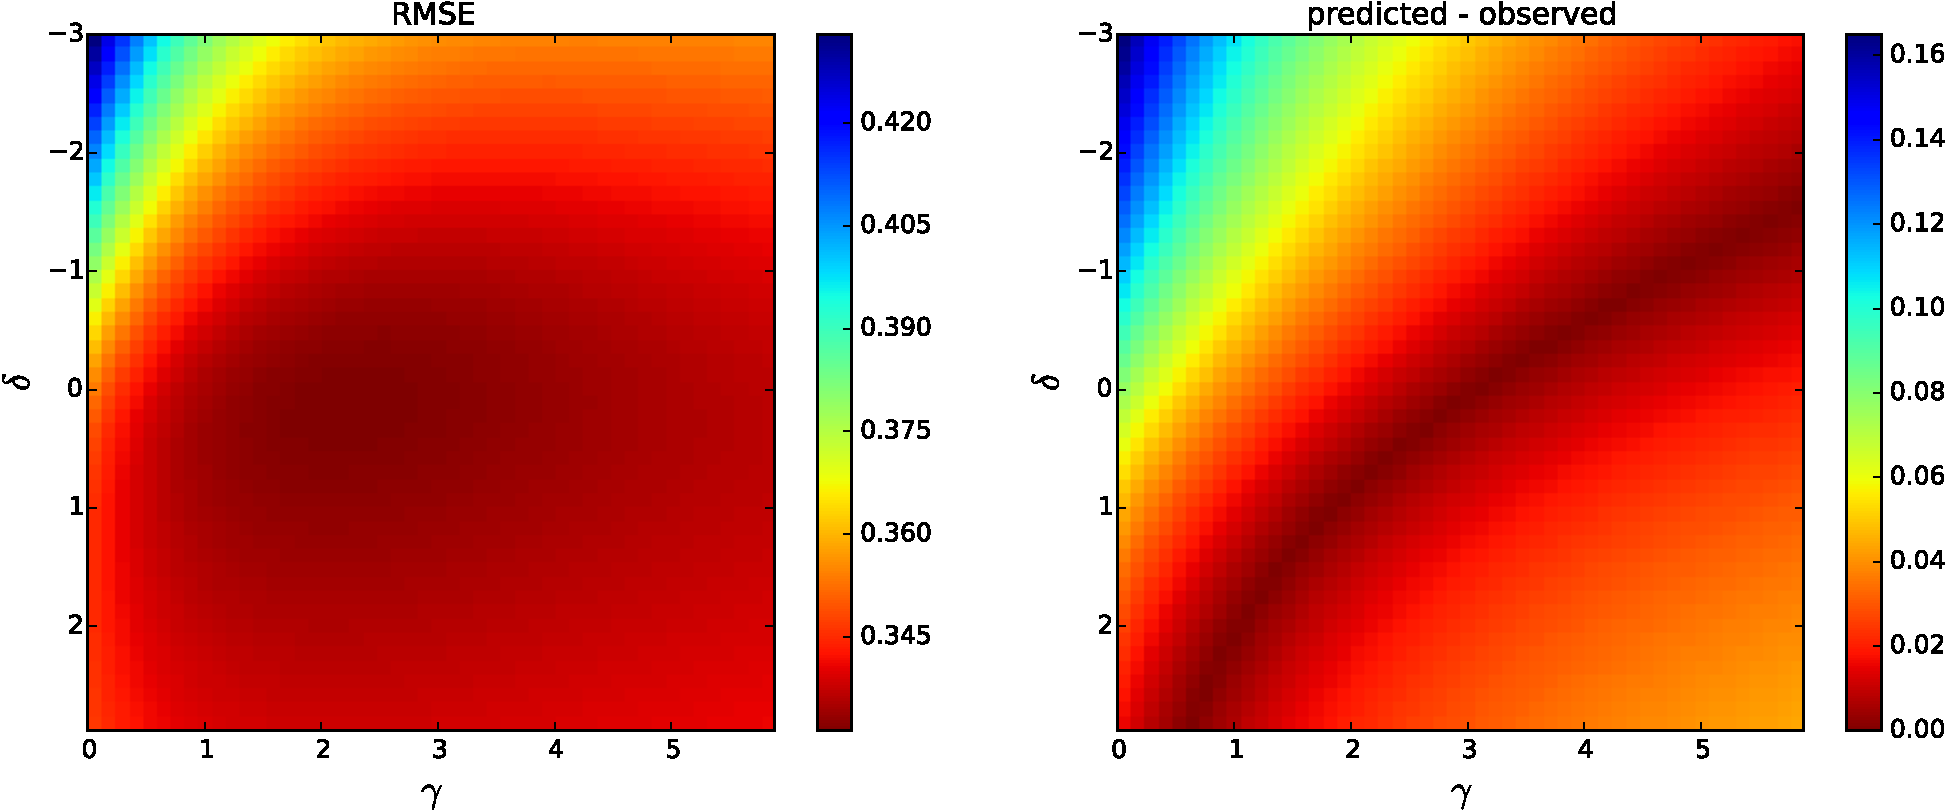
\includegraphics[width=\textwidth]{img/pfa-grid-search-rmse-off}
  \caption{Result of the grid search performed on the PFAE model with 2 parameters. The figure on the right hand size shows the averages of $p_i - y_i$ over all answers for a grid of parameters.}
  \label{fig-grid-search-rmse-off}
\end{figure}

Radek Pelánek in his work~\cite{Pelanek2015} figured out a better, more complicated way of parameter estimation which combines some aspects of gradient descent and is suitable in online learning. The update of parameters happens after arrival of every new data point (i.e. student's answer). This method is very practical particularly in our case where we need to find the most optimal and best calibrated time effect function. TODO: elaborate, properly describe the method and its applications, pseudocode

\section{Time Effect Functions}
\label{time-effect-functions}

In chapter~\ref{memory} we mentioned that forgetting usually respects the power law, which is often true in cases where the students have no prior knowledge of the practiced material. For our purpose, we have chosen the following functions with parameter $t$ representing the time of the last presentation and two parameters $a$ and $c$:

\begin{itemize}
  \item $f_{\mathit{log}}(t) = a - c \cdot \log(t)$
  \item $f_{\mathit{exp}}(t) = a \cdot e^{-c \sqrt{t}}$
  \item $f_{\mathit{poly}}(t) = a / t^c$
\end{itemize}

The shape of each of these time effect functions with logarithmically scaled $x$-axis is depicted on Figure~\ref{fig-time-effect-functions}.

\begin{figure}[htbp]
  \centering
  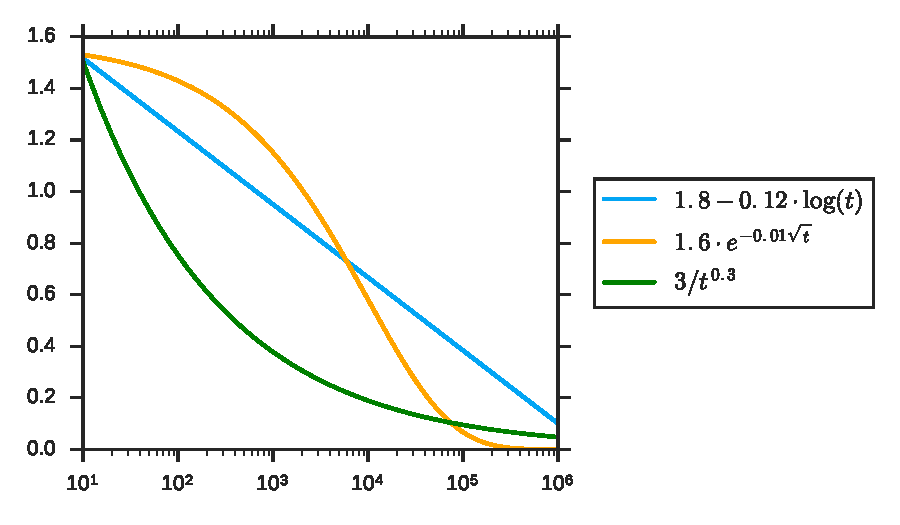
\includegraphics[width=\textwidth]{img/time-effect-functions}
  \caption{Candidates of time effect functions we inspected and evaluated in our analysis. Note that the $x$-axis is log scaled.}
  \label{fig-time-effect-functions}
\end{figure}

\subsection{The Staircase Function}
\label{staircase-function}

If we want to approximate the exact shape of a time effect function, we can define a staircase function with fixed intervals $\iota$. In each interval $(\iota_i, \iota_{i+1}]$, we preserve a learned value $a_i$ which represents an increase in memory activation. The formal definition of the staircase function $f_{\mathit{staircase}}$ is formalized in Equation~\ref{eq-staircase}.

\begin{equation} \label{eq-staircase}
  f_{\mathit{staircase}}(t) = \begin{cases}
            a_1, & \text{if } \iota_0 < t \leq \iota_1 \\
            a_2, & \text{if } \iota_1 < t \leq \iota_2 \\
                 & \hspace{1em} \dots \\
            a_n, & \text{if } \iota_{n-1} < t \leq \iota_n
         \end{cases}
\end{equation}

Applying simple linear algebra, we can further modify the staircase function so that the memory activation between two points is a linear function, this makes a better approximation of the learned values. The definition of the adjusted function is described in Equations~\ref{eq-staircase-iota-prime-definiton} and~\ref{eq-staircase-linear}, where $T$ is a set of all timing distances of all answers.

\begin{equation} \label{eq-staircase-iota-prime-definiton}
\begin{split}
  \hat{\iota}_0 &= \iota_0 \\
  \hat{\iota}_i &= \mathit{mean}\{t \in T~|~\iota_{i-1} < t \leq \iota_i\}
\end{split}
\end{equation}

\begin{equation} \label{eq-staircase-linear}
  f_{\mathit{staircase}}(t) = \begin{cases}
            a_1, & \text{if } \hat{\iota}_0 < t \leq \hat{\iota}_1 \\
            (t - \hat{\iota}_1) \frac{a_2 - a_1}{\hat{\iota}_2 - \hat{\iota}_1} + a_1, & \text{if } \hat{\iota}_1 < t \leq \hat{\iota}_2 \\
            \hspace{9em} \dots \\
            (t - \hat{\iota}_{n-1}) \frac{a_n - a_{n-1}}{\hat{\iota}_n - \hat{\iota}_{n-1}} + a_{n-1}, & \text{if } \hat{\iota}_{n-1} < t \leq \hat{\iota}_n     
         \end{cases}
\end{equation}

Note that $\hat{\iota}_0$ is in our case always equal to $0$ and $\hat{\iota}_n$ to infinity (in which case the memory activation in the interval is equal to $a_n$).

  \chapter{Evaluation and Analysis}

In the first part of this section we briefly depict the nature of the data set used for evaluation of the models and discuss some specifics of the implementation. In the next part we present the results of our analysis.

\section{Data Set}

For the analysis we used data from the online system for practicing geography\footnote{\url{http://www.slepemapy.cz}}~\cite{Papousek2014}. The data set contains more than 10~million answers from thousands of unique users~\cite{Papousek2015}. The data were filtered to contain only students with at least 50 answers and usually divided into 5 data sets, each containing at least 30 thousand answers. The answers of students who registered before the oldest question in the data set was answered were removed since it could temper with the results (considering we are interested primarily in models based on timing information).

\section{Toolchain}

The models were implemented in Python programming language. Experiments were performed in the Jupyter Notebook interactive environment\footnote{Jupyter Notebook is an open sourced web application for interactive computing, see~\url{https://jupyter.org/}}. Here is a list of the used libraries and modules:

\begin{itemize}
  \item SciPy, NumPy, Pandas
  \item Scikit-Learn
  \item Matplotlib
  \item NetworkX
\end{itemize}

\section{Response Time}

The response time of student to a question indicates how much well the item is learned. If the student answered quickly, almost automatically, it is very likely they either know the place very well or don't at all, depending on the correctness of their answer. On the other hand when the response is longer, the student is probably familiar with the item and might even recall the correct answer.

The Figure~\ref{fig-response-time} demonstrates the relationship between students' response time and the probability of recall. If the student's answer was suspiciously fast (response time is lower than 800 milliseconds), it usually means they are guessing. If the response time is between 1500 and 2000 milliseconds, it may indicate the student knows the correct answer.

Note that some places are bigger on the map then other, i.e. a question requiring the student to choose Russia on the map has generally lower response time than a question requiring to choose Andorra.

\begin{figure}[htbp]
  \centering
  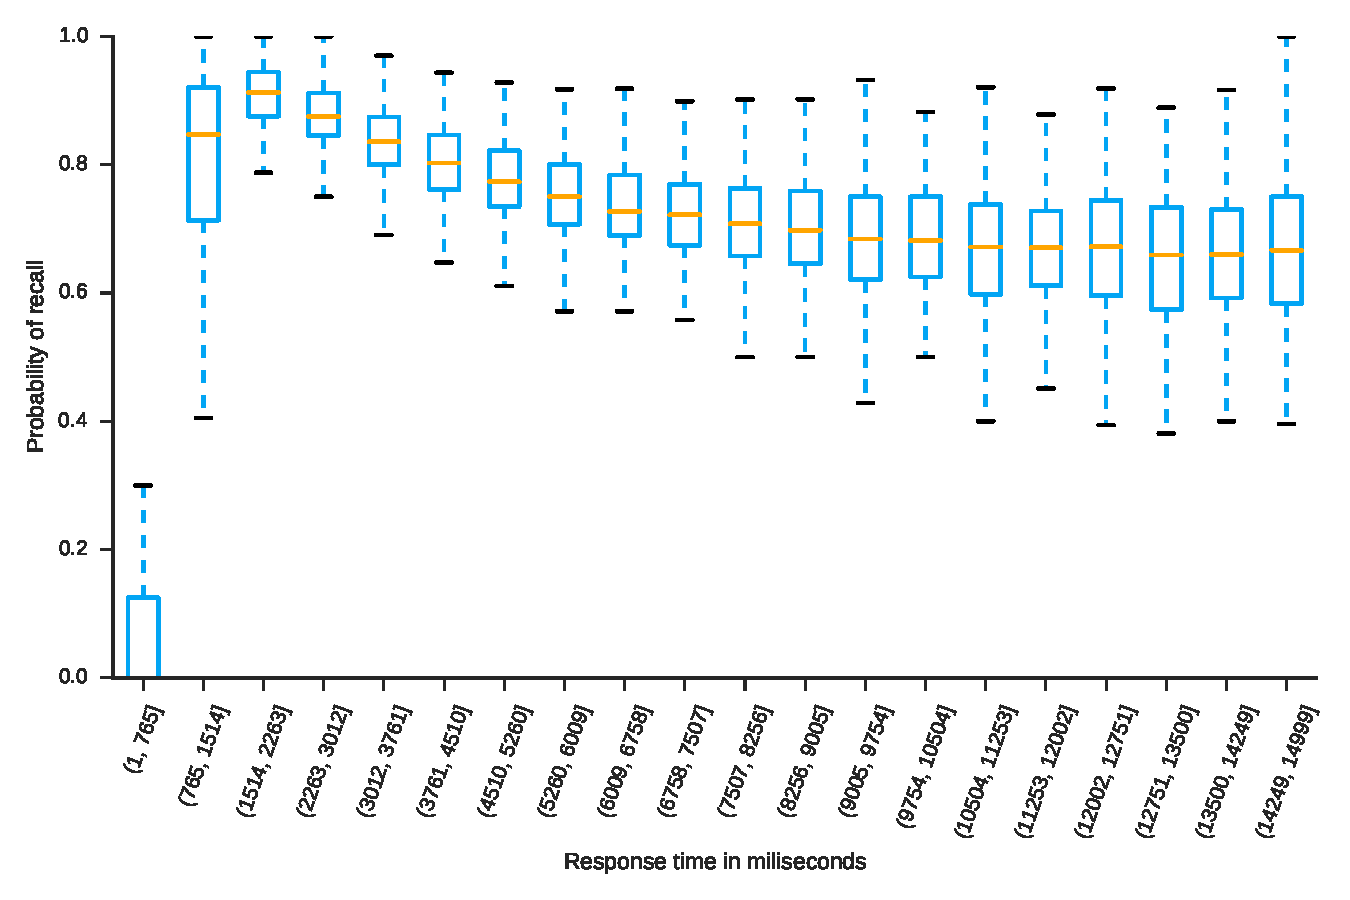
\includegraphics[width=\textwidth]{img/response-time}
  \caption{Relation between students' response time and probability of recall. Each box represents probabilities from all countries that belong in the relevant interval of response times.}
  \label{fig-response-time}
\end{figure}

\section{Calibration}

\section{Evaluation}

  \chapter{Conclusion}

TODO.


  \bibliography{references}
  \bibliographystyle{ieeetr}
\end{document}
